\documentclass{article}   

\usepackage[lighttt]{lmodern}
\usepackage{url}    
\usepackage{attachfile2}   
% \usepackage{natbib}
\usepackage{graphicx}
\usepackage{subcaption}
\usepackage[shortlabels]{enumitem}
\usepackage{placeins}
\usepackage{tabularx,ragged2e,booktabs,caption}
\usepackage{pdflscape}
\usepackage{tocbibind}
\usepackage{tocloft}
\usepackage{hyperref}
\usepackage[none]{hyphenat}
\usepackage{amsmath}
\usepackage{lscape}
\usepackage{booktabs}
\usepackage{afterpage}
\usepackage[margin=1in]{geometry}




\renewcommand{\abstractname}{\vspace{-\baselineskip}}
\DeclareTextFontCommand{\codefont}{\ttfamily \bfseries}
% \setcounter{secnumdepth}{-1}

\begin{document}

\title{WRF/EmWxNet High Resolution Nowcasting System v2.0\\ User Manual}
\author{Nadya Moisseeva}
\date{February 2016}    % type date between braces

\maketitle
\tableofcontents

\newpage
\section*{Introduction}
\addcontentsline{toc}{section}{Introduction}

WRF/EmWxNet High Resolution Nowcasting System has been developed to produce refined analysis fields by combining model forecast with real-time observations through downscaling and data assimilation. The current system relies on meteorological fields from Weather Research and Forecasting model (WRF) and observations from Emergency Weather Net Database (EmWxNet). This document is intended to provide an overview of the methods as well as user instructions for implementing the nowcasting system operationally. 

The \emph{User Guide}, contains setup instructions, overview of various system configurations and components, as well as a brief description of the output graphics. The \emph{Technical Description}, provides a more detailed review of the methods, analysis and its verification. 

\newpage
\section{Technical Description}
The \emph{Technical Description} provides a brief summary of the methods as well as a scientific rationale for their implementation. More importantly, it aims to explicitly highlight the underlaying simplifications and the potential limitations of WRF/EmWxNet High Resolution Nowcasting System design. The current analysis is limited to surface temperatures and precipitation only, however, will be expanded to include wind fields in the future. 

\subsection{Data and Domain Setup}

\noindent \textbf{DEM data}\\
High resolution (12arcsec, or $\approx$350m) DEM data were obtained from Natural Resources Canada Online Geospatial Data Extraction tool \cite{DEMdata}, available at \textbf{http://geogratis.gc.ca/site/eng/extraction}. The nowcasting system relies on the provided GeoTIFF format (georeferenced raster image in Geographic coordinate system). \\

\vspace{0.1cm}
\noindent \textbf{WRF model forecast fields}\\
The gridded first guess temperature, precipitation as well as lapse rate fields are produced from raw (non-postprocessed) WRF3-ARW NAM model runs, initialized daily at 0000UTC with NCEP data. The tested configuration used \textbf{d03} domain with 4km resolution. For precipitation analysis both the current and previous forecast hours are required to produce accumulated hourly precipition totatls. WRF 'RAINNC' variable for the previous hour is subtracted from the current analysis hour to get grid total hourly accumualated precipitation. \\

\vspace{0.1cm}
\noindent \textbf{EmWxNet observational data}\\
During each initialization of the analysis for a given forecast hour fresh observation data are pulled from the EmWxNet database. It is assumed that with any additional time more data could have been ingested into the database, which may improve the analysis (exception: no new EmWxNet data are loaded when system is ran in manual mode). 

All stations that fall within the user-specified domain bounds (excluding US territory) are extracted. The data are subsequently filtered to include only those measurements that fall within 5 minutes of the nowcast hour. If the allowed time range is extended, artifacts may be introduced into the analysis fields as neighboring stations reporting observations from opposite ends of the tolerance interval may produce conflicting readings. 

The observation stations are then quality-controlled by ensuring that the reported temperatures fall within a realistic range between -50 and +60 degrees C. For precipitation, reasonable amounts are expected to range between 0 and 100m for hourly totals. Lastly, the reliability of station metadata is tested by locating the DEM grid point closest to the listed station location and ensuring that the elevation discrepancy between the metadata altitude and DEM grid does not exceed 200m (typically 4-5 stations are excluded for the tested domain). 


\vspace{0.1cm}
\noindent \textbf{PRISM Precipitation Climatology}\\
High-resolution (~800m) precipitation climatology for years 1971-2000 for British Columbia were obtained from Pacific Climate Impacts Consortium (PCIC). 


\subsection{Downscaling Methods}
\subsubsection{Temperature}
Coarse (4km) first-guess temperature field (Figure \ref{fig:rawtemp}), produced from diagnostic \textbf{T2} variable in WRF output, are first interpolated to high resolution DEM grid. Due to frequent sharp gradients in temperature between land and water and the discrepancy between DEM and model coastlines, straight forward interpolation is insufficient and results in numerous artifacts and edge effects. Consequently, a split-interpolation solution is adopted. High-resolution landmask is generated for the given domain by classifying DEM points as land/water using the Python basemaps coastal polygons objects. Low-resolution model landmask is used to categorize model gridpoints. The latter are then interpolated separately to high-resolution grid, each spanning the entire DEM domain. The resultant fields are then masked with high resolution DEM landmask (removing water in land interpolation, and land in water interpolation) and concatenated together to produce a single high-resolution interpolated field. 

The next step is to interpolate model terrain elevation to high-resolution DEM grid. Since terrain smoothing is assumed to be applied to the majority of model runs no additional filtering is performed. 

Surface lapse rate is then calculated for each model grid point, using the user-specified number of model levels. A profile is constructed using temperature and level hight and profile slope is calculated for each grid point. During the course of the analysis several approaches were tested (using all surface temperature points from the model to produce a temperature profile; using observation temperatures only; subdividing the domain and several others). The alternatives fail to account for the high spatial variability in lapse rates across the domain. As can be seen in Figure \ref{fig:lapse}, areas shielded by mountains often show values close to dry lapse rate, while over-the-water and coastal regions have a substantially 'wetter' lapse rate. 

Similarly to height, the calculated model lapse rate field is interpolated to DEM grid. Lastly, the high-resolution interpolated temperature field is lapse-rate corrected, using the steps below for each DEM grid point:

\begin{eqnarray}
\Delta h = z_{DEM} - z_{interp} \nonumber \\
\Delta T = \Delta h * \gamma_{interp}/1000  \nonumber\\
T_{final} = T_{interp} + \Delta T
\end{eqnarray}
where $z$, $T$ and $\gamma$ are elevation, temperature and lapse rate, respectively. 

The resultant high-resolution temperature fields can be seen in Figure \ref{fig:downscaledT} in User Guide. 

\subsubsection{Precipitation}
Similarly to temperapture, the 1-hour adjusted precipitation totals are interpolated to high resolution DEM grid. As there are no sharp boundaries or interfaces in the precipitation data, split interpolation method is not necessary. No actual topographic adjustment is performed at this stage.  

\FloatBarrier
\subsection{Data Assimilation Methods}
\subsubsection{Temperature Data Assimililation}
EmWxNet temperature observations can be incorporated into the downscaled fields using two different methods: based on Region of Influence (ROI) and using Mother-Daughter (MD) approach. Both can be used to nudge the downscaled model first guess temperatures towards observations by either spreading the absolute observation value to nearby grids or by spreading the bias (or increment). Hence, four different configurations are possible. Based on a preliminary (and rather qualitative) assessment, the ROI method tends to perform better products in incremental mode, while MD assimilation scores higher by spreading the absolute observed value. Further, long-term testing would be necessary to determine, whether this assumption for all times of day/month/season. 

\subsubsubsection{Region of Influence (ROI)}
One of the biggest advantages of the ROI method is that it is not computationally expensive. The current configuration produces a domain with nearly two million grid points and approximately 200 observation stations - sufficient to substantially increase the nowcast time delay. While nearest-neighbor search on such a large domain is typically a difficult computational task, the current analysis uses multiple passes of KD-tree algorithm \cite{KDtrees} to identify grids affected by observations, based on user-defined horizontal region of influence. Once the grid points are identified the temperature field is corrected using a basic inverse-distance weighing scheme in three dimensions (using user-specified vertical ROI for elevation adjustment).\\

\noindent\textbf{In incremental mode:}\\
Let $X$ be 2-dimensional vector corresponding to a grid point location. Then for each grid point $X_i = (x_i,y_i)$, affected by one or more observation stations at $X_j = (x_j,y_j)$, we can calculate a weighted adjustment. In the horizontal:
\begin{eqnarray}
Dh_{ij} = | X_{i} - X_{j} | \nonumber\\ 
Wh_{ij} = (\frac{(r - Dh_{ij})}{r})^2 \nonumber
\end{eqnarray}
where $Dh$, $Wh$ and $r$ are horizontal distance, horizontal weight and user-defined horizontal radius of influence, respectively. 

In the verital:
\begin{eqnarray}
Dv_{ij} = | z_{f}(x_i,y_i) - z_{obs}(x_j,y_j) | \nonumber\\
Wv_{ij} = (\frac{(r_e - Dv_{ij})}{r_e})^2 \nonumber
\end{eqnarray}
where $Dv$, $Wv$, $z$ and $r_e$ denote vertical distance, vertical weight, elevation, and user-defined vertical ROI tolerance, respectively. 

The total weight $Wt_{ij}$ is simply:
\begin{equation}\label{eq:Wt}
Wt_{ij} = Wh_{ij} * Wv_{ij}\\
\end{equation}

If $T$ is the 2m temperature and subscripts $obs$ and $f$ denote values from observation stations and downscaled forecast, we can compute the final adjusted grid point value $T_i(x_i,y_i)$ by recursively correcting the forecast with a weighed bias for each station $j$.
\begin{eqnarray}
\Delta T_{ij} = T_{obs}(x_j,y_j) - T_{f}(x_j,y_j) \nonumber\\ 
T_i = T_f(x_i,y_i) + \Delta T_{ij} * Wt_{ij}
\end{eqnarray}
\\

\noindent\textbf{In temperature-adjustment mode:}\\
Alternatively, rather than correcting temperature increments, it is possible to spread lapse-rate adjusted observation temperature values. Using Eq. \ref{eq:Wt} to calculate the total weight and model lapse rate $\gamma_{interp}$ to calculate $T_i$:
\begin{eqnarray}
T_i = T_f(x_i,y_i) * (1-Wt_{ij}) + (T_{obs}(x_j,y_j)+ \frac{Dh_{ij}*\gamma_{i}(x_i,y_i)}{1000})*Wt_{ij}
\end{eqnarray}
\\
The main drawback of this approach is that for days with a notable discrepancy between model and observations (i.e. for "bad" forecasts) the correction is prone to producing a so-called bull's eye effect. While statistically the verification scores are still likely to show improvement, the output fields will present an unphysical visual pattern. In such cases the Mother-Daughter approach discussed next is, without a doubt, the superior choice for data assimilation.

\subsubsubsection{Mother-Daughter (MD)}
The utility of the MD approach was first demonstrated for surface temperature analyses by Deng \emph{et al} (\cite{Deng2005}), and was shown to outperform other schemes over mountainous and coastal terrain. The main challenge with this method is the computational load of calculating sharing factors for the large number of stations in high resolution grid space. As mentioned earlier, in an attempt to mitigate this problem the current system builds a database of station sharing factors and anisotropic distances for each user-defined set of MD parameters, and appends it as necessary. The weight adjustment $W_{ij}$ for grid point $i$ due to observation station $j$ is calculated as follows:

\begin{eqnarray}
W_{ij} = (\frac{D_{max} - D_{ij}}{D_{max}})^2 * S_{ij}
\end{eqnarray}
where $D_{max}$ is the user-defined maximum distance cutoff (\textbf{cutoff\_dist}), $D_{ij}$ is the MD anisotropic distance to from $X_j$ to $X_i$ and $S_{ij}$ is the MD sharing factor. An example of the spread of influence of a subset of observation stations can be seen in Figure \ref{fig:MD}.

The temperature field is then adjusted in either incremental or absolute mode. Similarly to ROI method to produce $T_{ij}$, bias is simply added to the forecast temperature field, while in absolute mode the observation temperature is lapse-rate adjusted to each grid-point height. Lastly, to compute the combined effects of all stations in MD mode for grid point $i$:

\begin{eqnarray}
T_i = \frac{(1 * T_f(x_i,y_i) + \sum\limits_{j=1}^n \Delta T_{ij} * W_{ij})}{1 + \sum\limits_{j=1}^n W_{ij}}
\end{eqnarray}

\newgeometry{left=1cm}
\begin{landscape}
\pagestyle{empty}

\begin{figure}
\makebox[\textwidth][c]{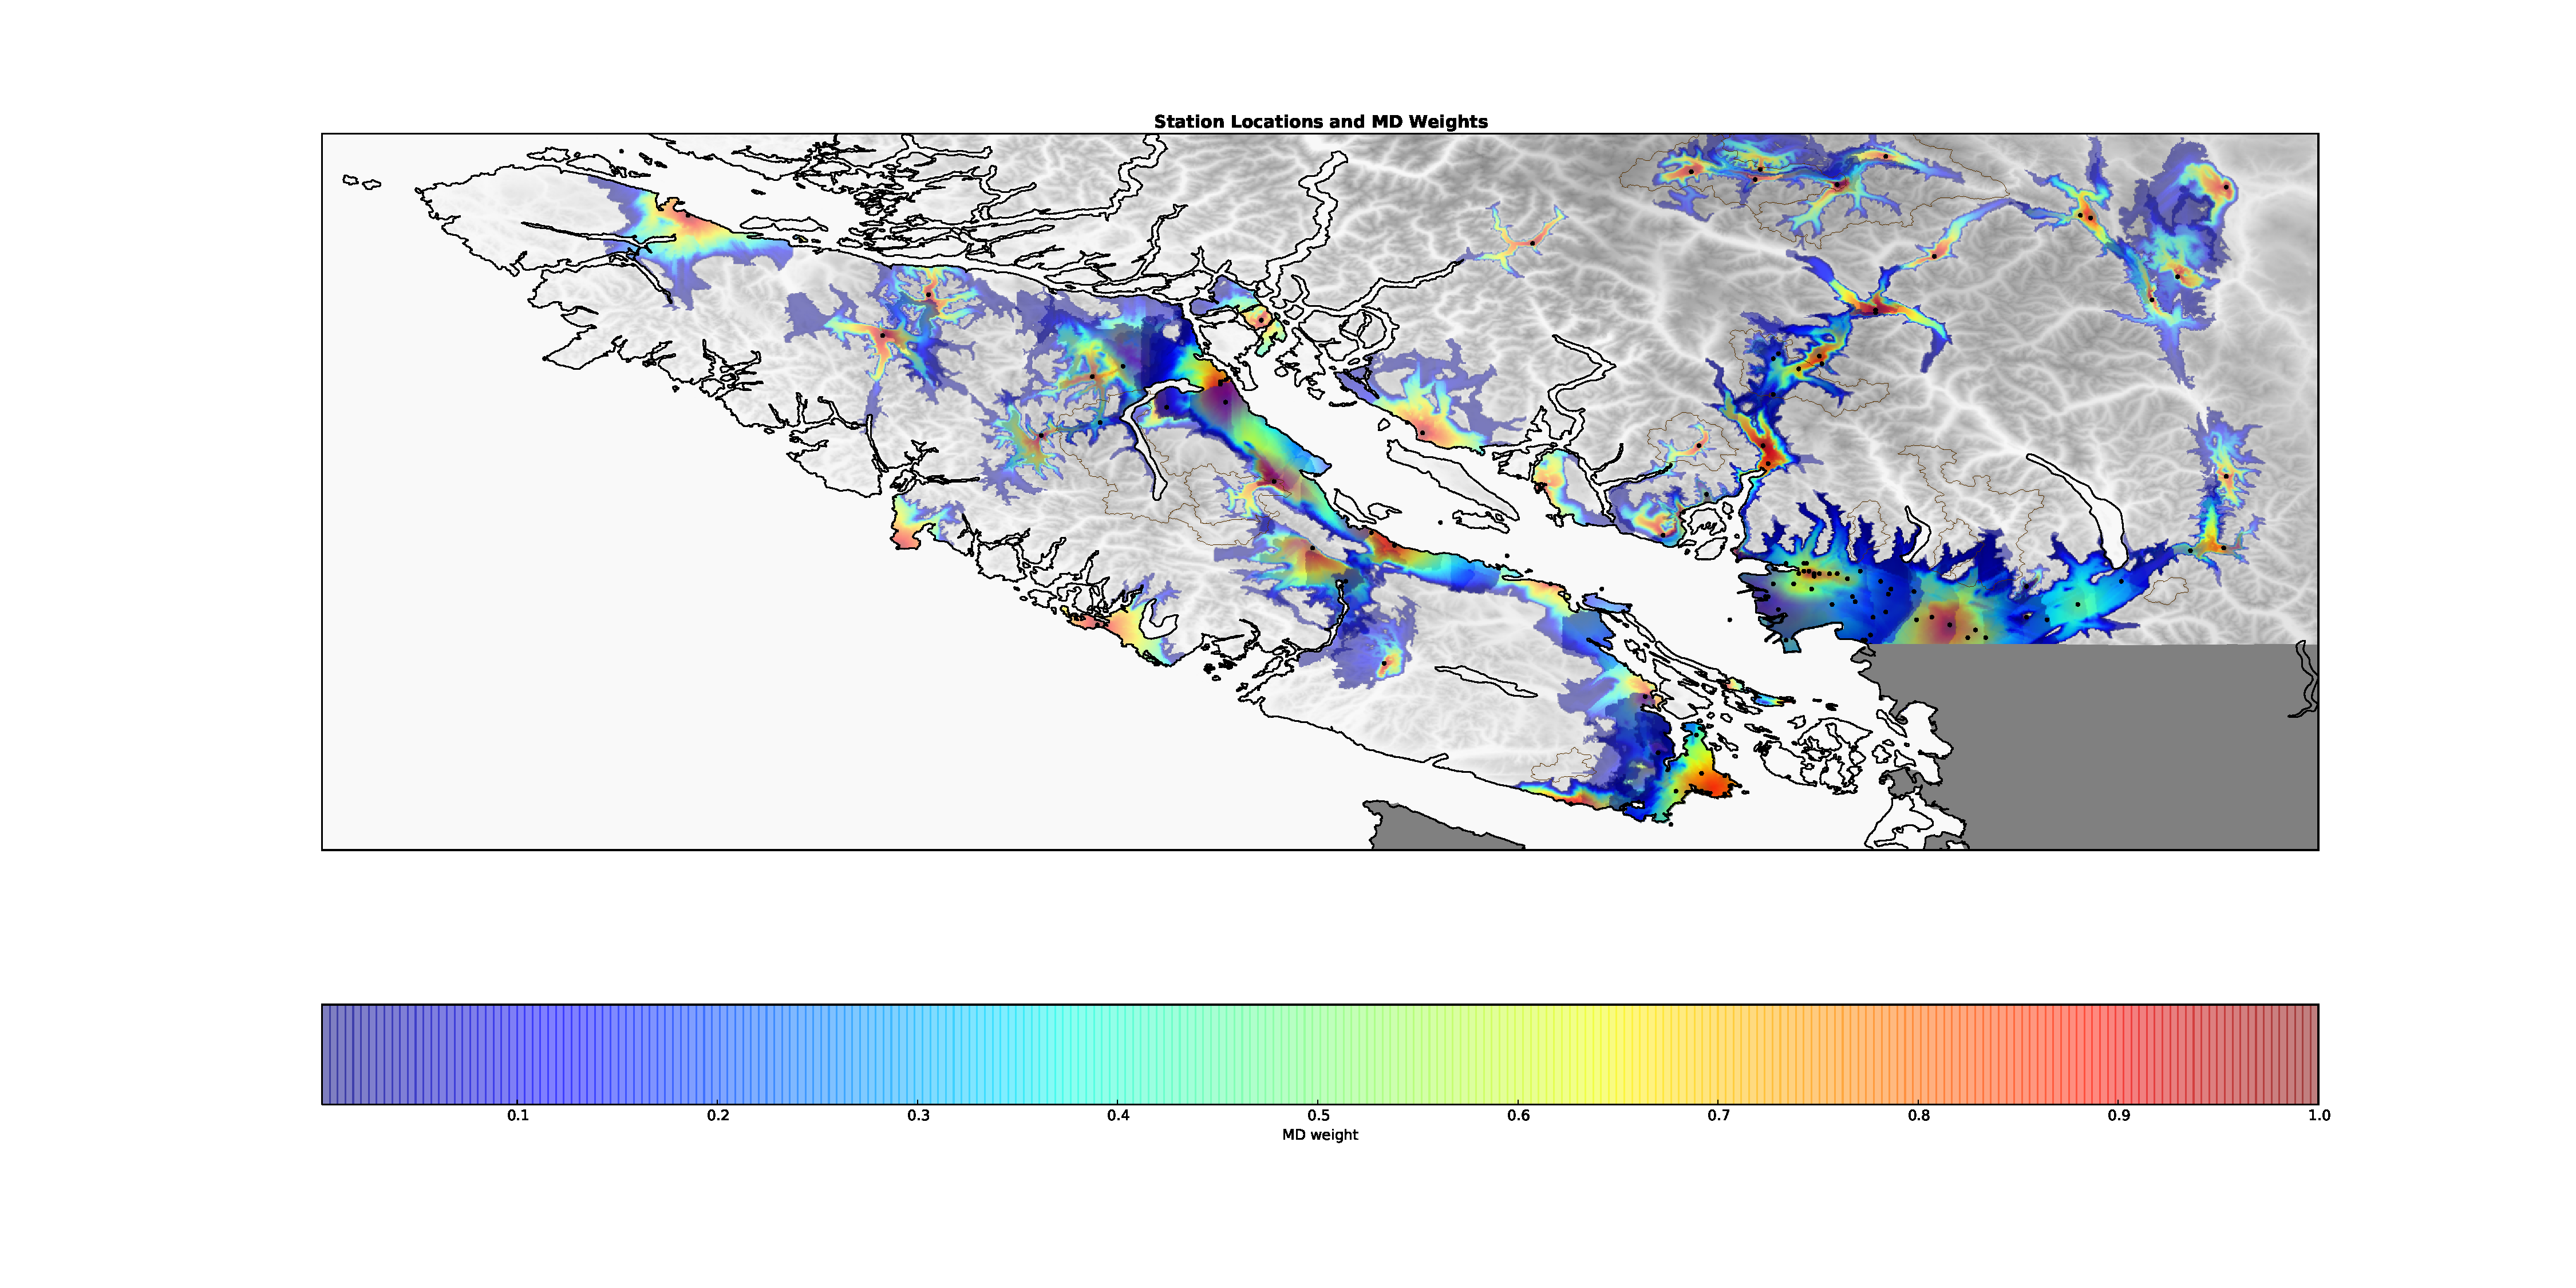
\includegraphics[width=12in]{./graphics/md_weights_current_run.pdf} }
\caption{Observation stations and the strength of their influence on surrounding gridpoints	 (shown for a subset of stations only)}\label{fig:MD} 
\end{figure}

\end{landscape}
\restoregeometry
\pagestyle{plain}

\subsubsection{Precipitation}

\FloatBarrier

\subsection{Verification}
Evaluation of each run is embedded in the code and is performed for both downscaling and data assimilation analysis components. Any on-water points are excluded from evaluation to avoid edge effects and errors due to land/water classification differences between the model, DEM grid and basemaps. Figure \ref{fig:verifDS} is an example of standard graphical output for downscaling verification. All available land points are used for the scatter plots and statistical metric calculations. Generally, for days with fairly accurate first-fuess forecast fields, downscaling alone produces a measurable improvement in verification statistics. 

Final analysis fields produced through downscaling and data assimilation are assessed using cross-evaluation with an independent test dataset. Corrections are performed for a user-defined fraction of stations, randomly selected from available observation locations (training subset), and subsequently evaluated with the remaining subset of test stations. Statistical metrics included in the output plot (Figure \ref{fig:verifDA}) are similarly based on the test data only. 

\newpage
\section{User Guide}
\subsection{Code Components}

\FloatBarrier
Figure \ref{fig:flowchart} shows the various components of the nowcasting system. While the majority of the analysis is performed using Python language (as denoted by *.py file extensions), the primary operational driver and EmWxNet databased wrapper are coded and bash shell (*.bash) and C (*.exe), respectively. 

Note, that only one of the components, namely \textbf{da\_config.py}, is to be modified by the user. The remainder of the system is controlled by the main bash and python drivers automatically. While unnecessary for day-to-day operation of the nowcasting system the primary details and functions of each component are described below. 

\begin{figure}[hb]
\centering
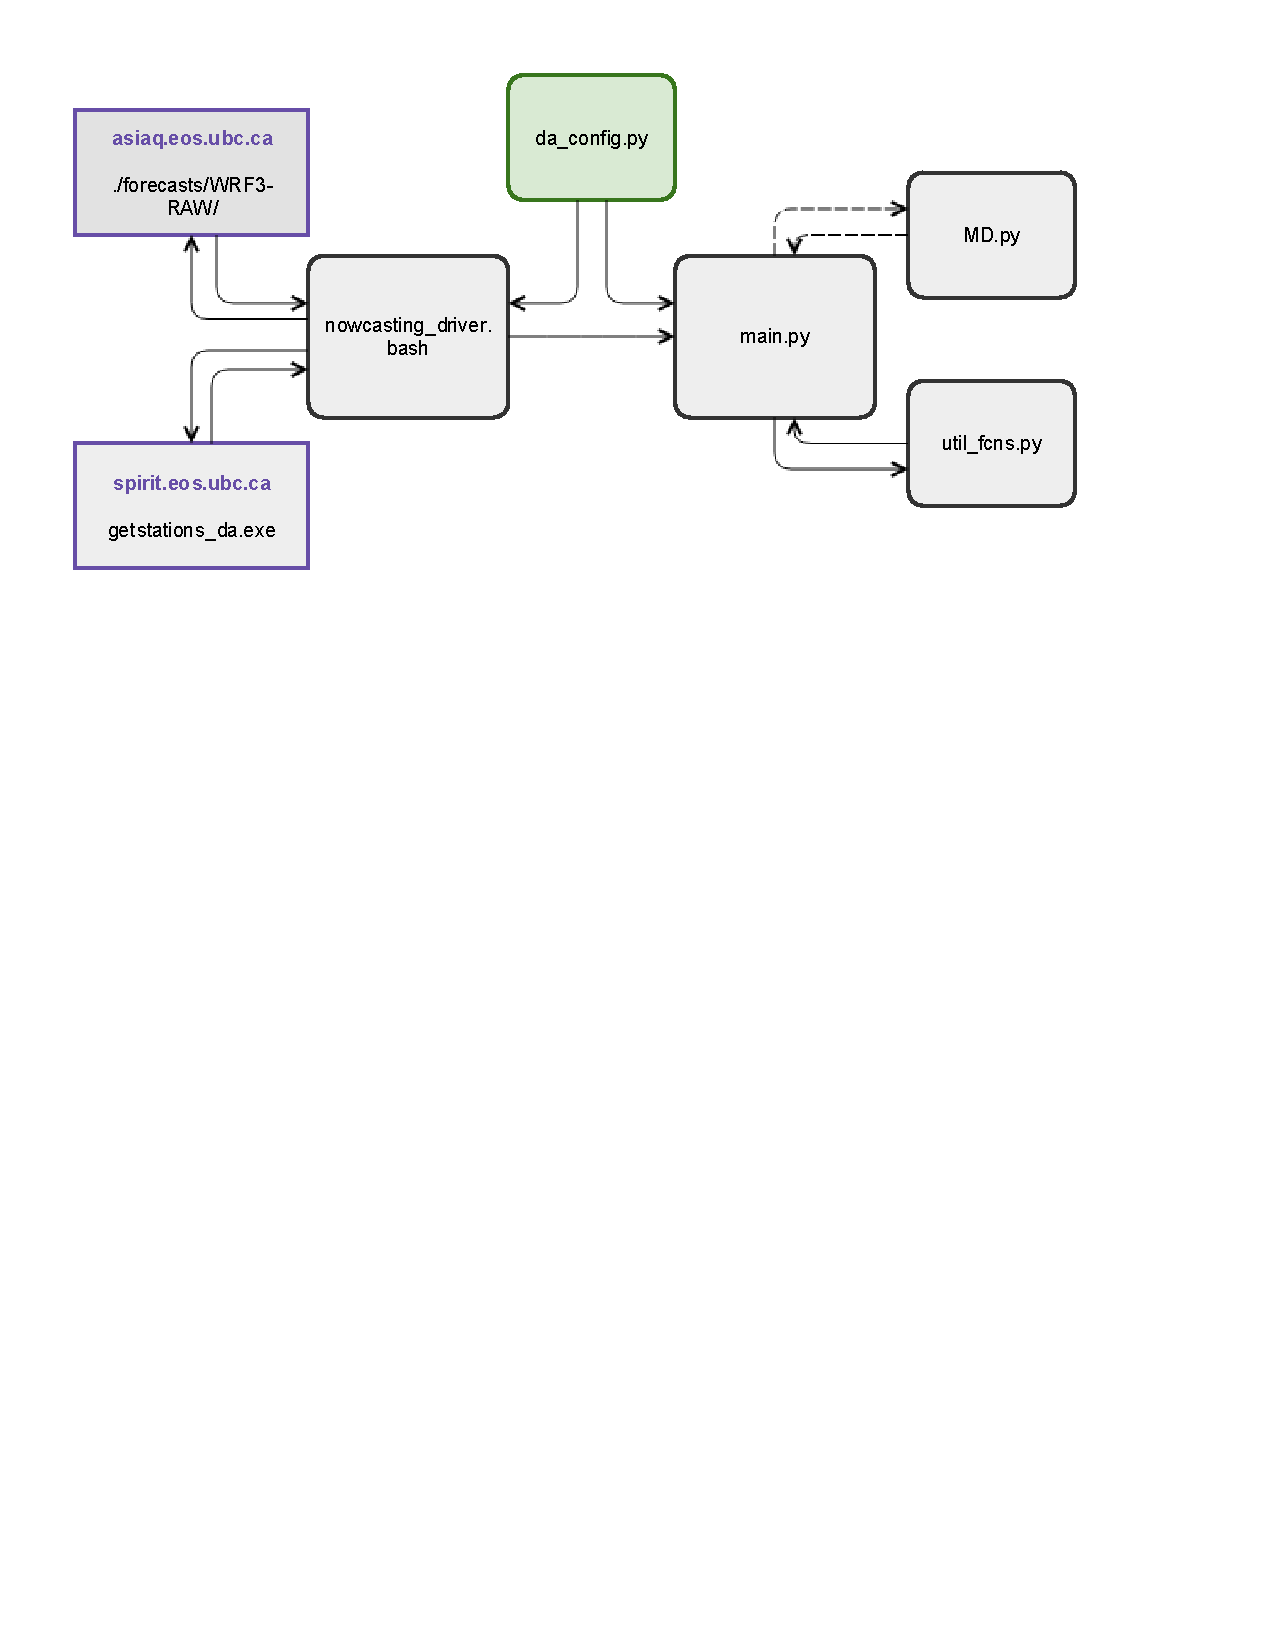
\includegraphics[width=6in]{./graphics/CodeFlowchart.pdf} 
\caption{Nowcasting system flowchart. Remote servers typeset in purple; user-controlled component (\textbf{da\_config.py}) shown in green}\label{fig:flowchart}
\end{figure}
\FloatBarrier


\vspace{0.3cm}
\noindent \textbf{da\_config.py}\\
Python equivalent of the namelist: contains all of the user-controlled settings. For details of the included variables and parameters refer to Section \ref{sec:config}. 

\vspace{0.3cm}
\noindent \textbf{nowcasting\_driver.bash}\\
Bash shell script: drives all of the main system components, including connection to remote servers, moving of files to local computer and initialization of python routines. 
\begin{itemize}[noitemsep]\vspace{-2mm}
	\item Locates required forecast WRF data; moves raw netcdf files from \textbf{asiaq.eos.ubc.ca} server if necessary
	\item Extracts EmWxNet data from \textbf{spirit.eos.ubc.ca} and creates copies on the local computer
	\item Runs the main Python analysis driver
\end{itemize}

\vspace{0.3cm}
\noindent \textbf{main.py}\\
Main Python analysis driver: 
\begin{itemize}[noitemsep]\vspace{-2mm}
	\item Constructs analysis domain (creates basemaps and landmasks, if necessary) 
	\item Interpolates model data to Digital Elevation Model (DEM) resolution
	\item Performs data downscaling
	\item Performs data assimilation
	\item Produces output graphics
\end{itemize}
May be used as part of an operational system controlled by \textbf{nowcasting\_driver.bash} or independently. 

\vspace{0.3cm}
\noindent \textbf{getstations\_da.exe}\\
C-based code wrapper for pulling observations from EmWxNet. Note (!): lat/lon extent of the area for which the observations are extracted is currently hard-coded in the file (includes southern BC only). The domain extent can easily be changed in the input header within the file. It should be equivalent or larger than the domain used for nowcasting (unnecessary stations will be excluded).

\vspace{0.3cm}
\noindent \textbf{MD.py}\\
Mother-Daughter data assimilation script for calculating sharing factors for observation stations. Builds a weights/distances database for observation stations, appends stations as necessary.

\vspace{0.3cm}
\noindent \textbf{PRISM.py}\\
PRISM-based data assimilation script for calculating regions of precipitation influence for observation stations. Builds a weights database for observation stations, appends stations as necessary.

\vspace{0.3cm}
\noindent \textbf{util\_fcns.py}\\
Python utility module: contains all of the subroutines called by the main Python driver. 


\subsection{System Requirements}
Required languages for the local computer (excludes requirements for remote servers, C-compilers, etc.)\\

1. \textbf{Unix bash shell}. Note (!): GNU-based Linux shell uses a different version of the \textbf{date} command, which may not have the same flags as those required by the current operational setup. \\

2. \textbf{Python 2.7}, to be tested with Python 3.4. Primary packages, including NumPy, matplotlib, SciPy

\subsection{Setup}

This section describes the initial setup of the system. These steps do not need to be repeated for any subsequent new analysis/domain configurations and are only performed once. 
\begin{enumerate}[1.]
\item Create a new folder for storing the code. \\ Download the contents of \textbf{http://gl.tawhiri.eos.ubc.ca/nmoisseeva/nowcasting} to the new folder.
\item Establish keychain access to \textbf{spirit}. Ensure that you are able to ssh and copy files from the server without manual password entry. 
\item Mount the \textbf{asiaq} forecasts folder as a shared drive (MacOS). For Linux installations, modify the \textbf{nowcasting\_driver.bash} to use ssh and scp with keychain access. 
\item Copy the contents of \textbf{./emx} subfolder to \textbf{spirit.eos.ubc.ca}. Ensure that the domain specified in the input header of \textbf{getstations\_da.c} is the same or larger than the one that will be analyzed. Build the C code using the provided \textbf{makefile}. A successful compilation will produce a \textbf{getstations\_da.exe} file. 
\item Verify all paths and user names input header of \textbf{nowcasting\_driver.bash}, save updates. 
\item Configure \textbf{config\_da.py} (refer to Section \ref{sec:config}) and run analysis (refer to Section \ref{sec:run})

\end{enumerate}

\subsection{User Configuration}\label{sec:config}

Following the initial setup of the nowcasting system, the domain and analysis configuration can be changed by simply modifying the settings in \textbf{da\_config.py}. The options and flags along their with their functionality are described below. \\

\noindent- - - - - - - - - - - - - - - - - - - - - - - - - - - - - - - -\\
\noindent\#defining input and output locations and source files\\

\noindent \textbf{fig\_dir}\\
Path to folder for storing output graphics

\vspace{0.1cm}
\noindent \textbf{netcdf\_dir}\\
Path to storage folder for raw WRF netcdf data from the model. 

\vspace{0.1cm}
\noindent \textbf{netcdf\_prefix}\\
The name format (without timestamp) of the raw WRF netcdf file. 

\vspace{0.1cm}
\noindent \textbf{emx\_dir}\\
Path to storage folder for EmWeatherNet data. 

\vspace{0.1cm}
\noindent \textbf{geotiff}\\
Name of the GeoTIFF file containing the DEM data for the domain.  

\vspace{0.1cm}
\noindent \textbf{landmask\_dir}\\
\emph{Optional}: Path to folder containing numpy landmask. 

\vspace{0.1cm}
\noindent \textbf{basemap\_dir}\\
\emph{Optional}: Path to folder containing numpy basemap. 

\vspace{0.1cm}
\noindent \textbf{emx\_name}\\
\emph{Changes not recommended}: Name of output file from getstations\_da.c. Leave unchanged, unless altered in C code. 

\vspace{0.5cm}
\noindent- - - - - - - - - - - - - - - - - - - - - - - - - - - - - - - -\\
\noindent\#domain configuration\\

\noindent \textbf{lat}\\
\lbrack minimum lat, max latitude\rbrack

\vspace{0.1cm}
\noindent \textbf{lon}\\
\lbrack min longitude, max longitude\rbrack


\vspace{0.5cm}
\noindent- - - - - - - - - - - - - - - - - - - - - - - - - - - - - - - -\\
\noindent\#data assimilation configuration\\

\noindent \textbf{run\_MD}\\
Flag to use Mother-Daughter approach: 1 for MD data assimilation; 0 for ROI data assimilation

\vspace{0.1cm}
\noindent \textbf{verif\_frac}\\
Fraction of data that will be used for model training: the remainder will be used for cross evaluation. 

\vspace{0.1cm}
\noindent \textbf{bias\_mode}\\
Flag to correct temperature increments: 1 for incremental (bias) correction; 0 for absolute temperature correction

\vspace{0.1cm}
\noindent \textbf{delay\_hr}\\
For operational use: analysis delay (in hours)

\vspace{0.5cm}
\noindent- - - - - - - - - - - - - - - - - - - - - - - - - - - - - - - -\\
\noindent\#ROI DA configuration\\

\noindent \textbf{roi}\\
Horizontal range of influence for ROI-based data assimilation (in decimal degrees)

\vspace{0.1cm}
\noindent \textbf{elev\_roi}\\
Vertical range of influence for ROI-based data assimilation (in meters)



\vspace{0.5cm}
\noindent- - - - - - - - - - - - - - - - - - - - - - - - - - - - - - - -\\
\noindent\#MD DA configuration\\

\noindent \textbf{params}\\
$a$,$b$,$Z_{ref1}$,$Z_{ref2}$ Parameters for calculating MD sharing factors

\vspace{0.1cm}
\noindent \textbf{dist\_cutoff}\\
Maximum anisotropic horizontal distance in degrees (when reached, ending iteration)

\vspace{0.1cm}
\noindent \textbf{weight\_cutoff}\\
Minimum change in MD weight values required to continue iteration


\vspace{0.5cm}
\noindent- - - - - - - - - - - - - - - - - - - - - - - - - - - - - - - -\\
\noindent\#temperature and lapse rate configuration\\

\noindent \textbf{lvl}\\
Number of model levels to use for lapse rate calculation (starting from surface)

\vspace{0.1cm}
\noindent \textbf{T\_range}\\
Fixed colormap range to use for output temperature plots (in C, centered at 0)


\subsection{Ways to Run the Analysis}\label{sec:run}
The nowcasting analysis can be performed in an automated as well as manual mode. Usage instructions for both approaches are described below. Note that the first-time run (whether automated or manual) for a new domain/settings may take a substantial amount of time ($\approx$7-10 min), as new basemaps, landmasks and (optionally) MD/PRISM weights are being calculated. The code is optimized to store the output of these time-consuming operations and allow recycling for subsequent runs. 

\subsubsection{Operational/Automated Mode}
When ran operationally, the flow of the analysis is controlled by \textbf{nowcasting\_driver.bash} shell script. All the required process flow settings are passed here from \textbf{da\_config.py} automatically. Based on the user-specified time delay the bash script will copy all the necessary files from remote serves, store them in automatically generated subdirectories (by date) and run the main analysis. Note (!): all timestamps are UTC. \\

\noindent \emph{For a single automated run:} 
\begin{enumerate}[1.]
\item In terminal, navigate to your local nowcasting folder. 
\item Modify \textbf{da\_config.py} to desired settings.
\item In terminal, type: \textbf{bash nowcasting\_driver.bash}\\
\end{enumerate}
\noindent \emph{For a repeated automated run:} \\
\noindent Schedule a task to your \textbf{crontab} to call  \textbf{bash nowcasting\_driver.bash} with desired frequency\\

\subsubsection{Manual Mode}
The Python analysis component (\textbf{main.py}) may be ran as a stand-alone code with existing datasets, without evoking connections to remote servers. \\

\noindent \emph{For a single manual run:} \\
\begin{enumerate}[1.]
\item In terminal, navigate to your local nowcasting folder. 
\item Modify \textbf{da\_config.py} to desired settings. Note that in manual mode \textbf{delay\_hr} variable is ignored. 
\item Ensure that raw model and observation data are located in \textbf{./year/month/day/hr} subdirectories of \textbf{netcdf\_dir} and \textbf{emx\_dir}, respectively.
\item In terminal, type: \\
\textbf{python main.py filename}\\
 where \textbf{filename} is the full name of the raw netcdf file, including prefix and timestamp
\end{enumerate}

\subsection{Output Graphics}
\FloatBarrier
The final product of the analysis consists of high resolution field plots, verification graphs, as well as several auxiliary graphics. These are stored in  \textbf{./year/month/day/hr} subdirectory within the user-specified \textbf{fig\_dir}. Sample images and their brief descriptions are shown below. 

\newgeometry{left=1cm}
\begin{landscape}
\pagestyle{empty}

\begin{figure}
\makebox[\textwidth][c]{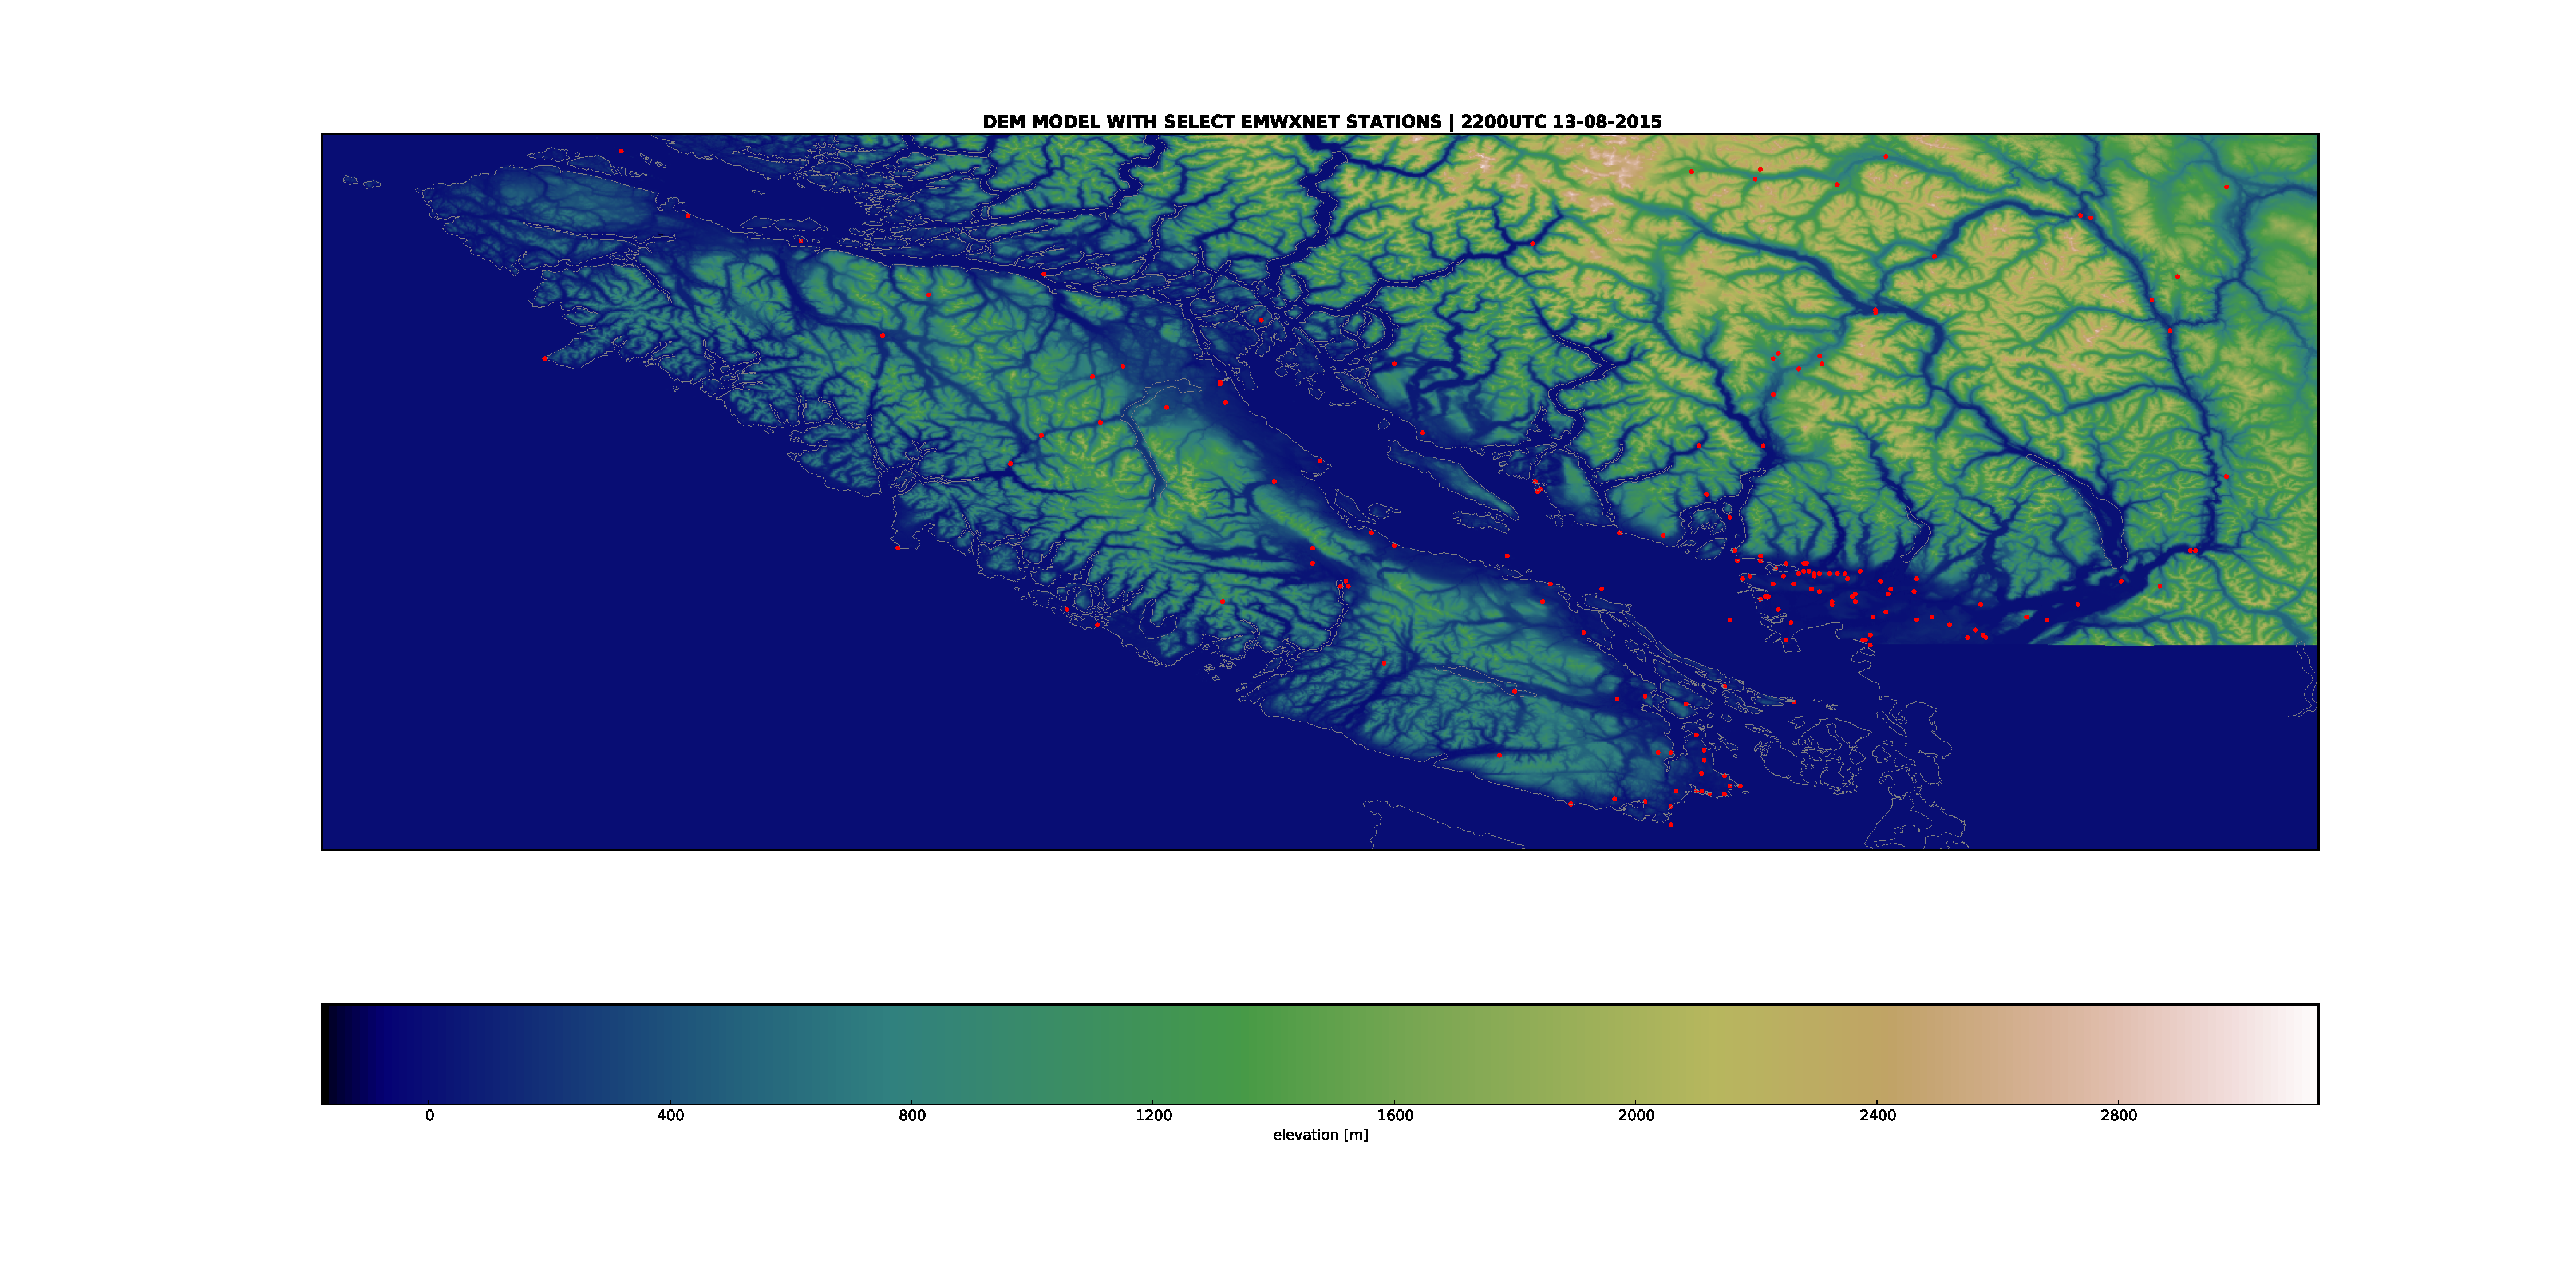
\includegraphics[width=12in]{./graphics/DEM_obs_12arcsec_2015-08-13_22.pdf} }
\caption{Analysis domain with 12arcsec DEM data. Select EmWxNet stations with observations for 2015-08-13 2200 UTC shown as red scatter.}\label{fig:dem} 
\end{figure}

\begin{figure}
\makebox[\textwidth][c]{\includegraphics[width=12in]{./graphics/temp_raw_2015-08-13_22.pdf} }
\caption{Raw 2m temperature fields from WRF netcdf output (4km resolution).}\label{fig:rawtemp} 
\end{figure}

\begin{figure}
\makebox[\textwidth][c]{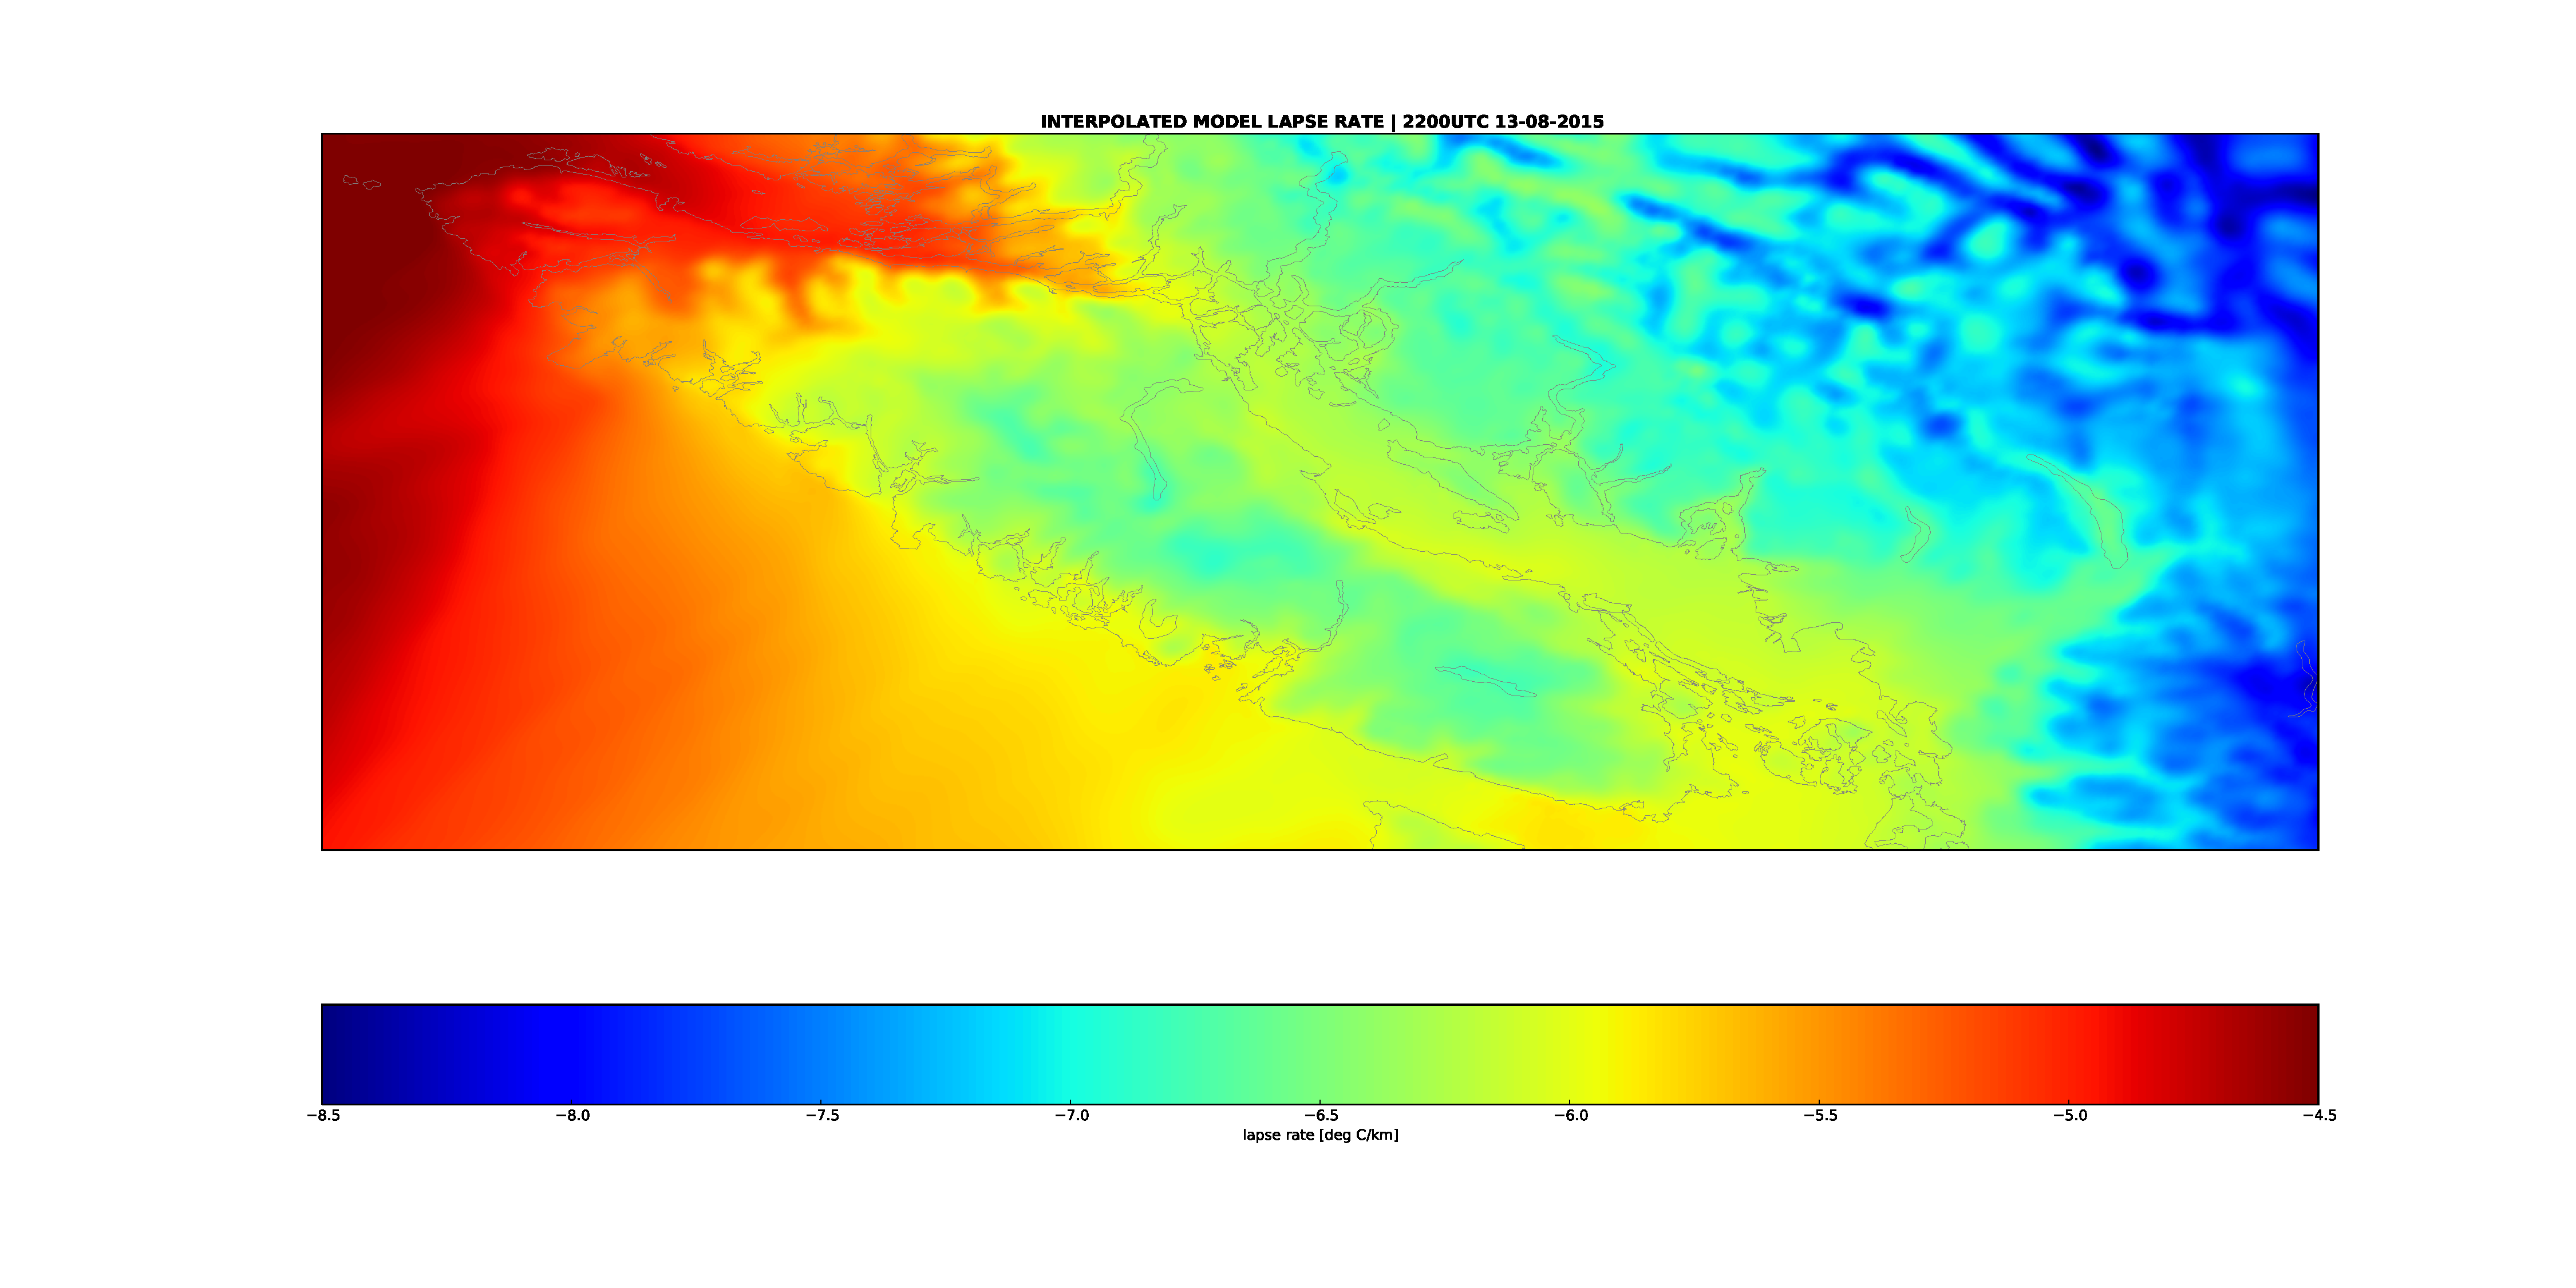
\includegraphics[width=12in]{./graphics/lapse_rate_2015-08-13_22.pdf} }
\caption{Raw WRF model lapse rate, based on first 20 layers about the surface.}\label{fig:lapse}
\end{figure}

\begin{figure}
\makebox[\textwidth][c]{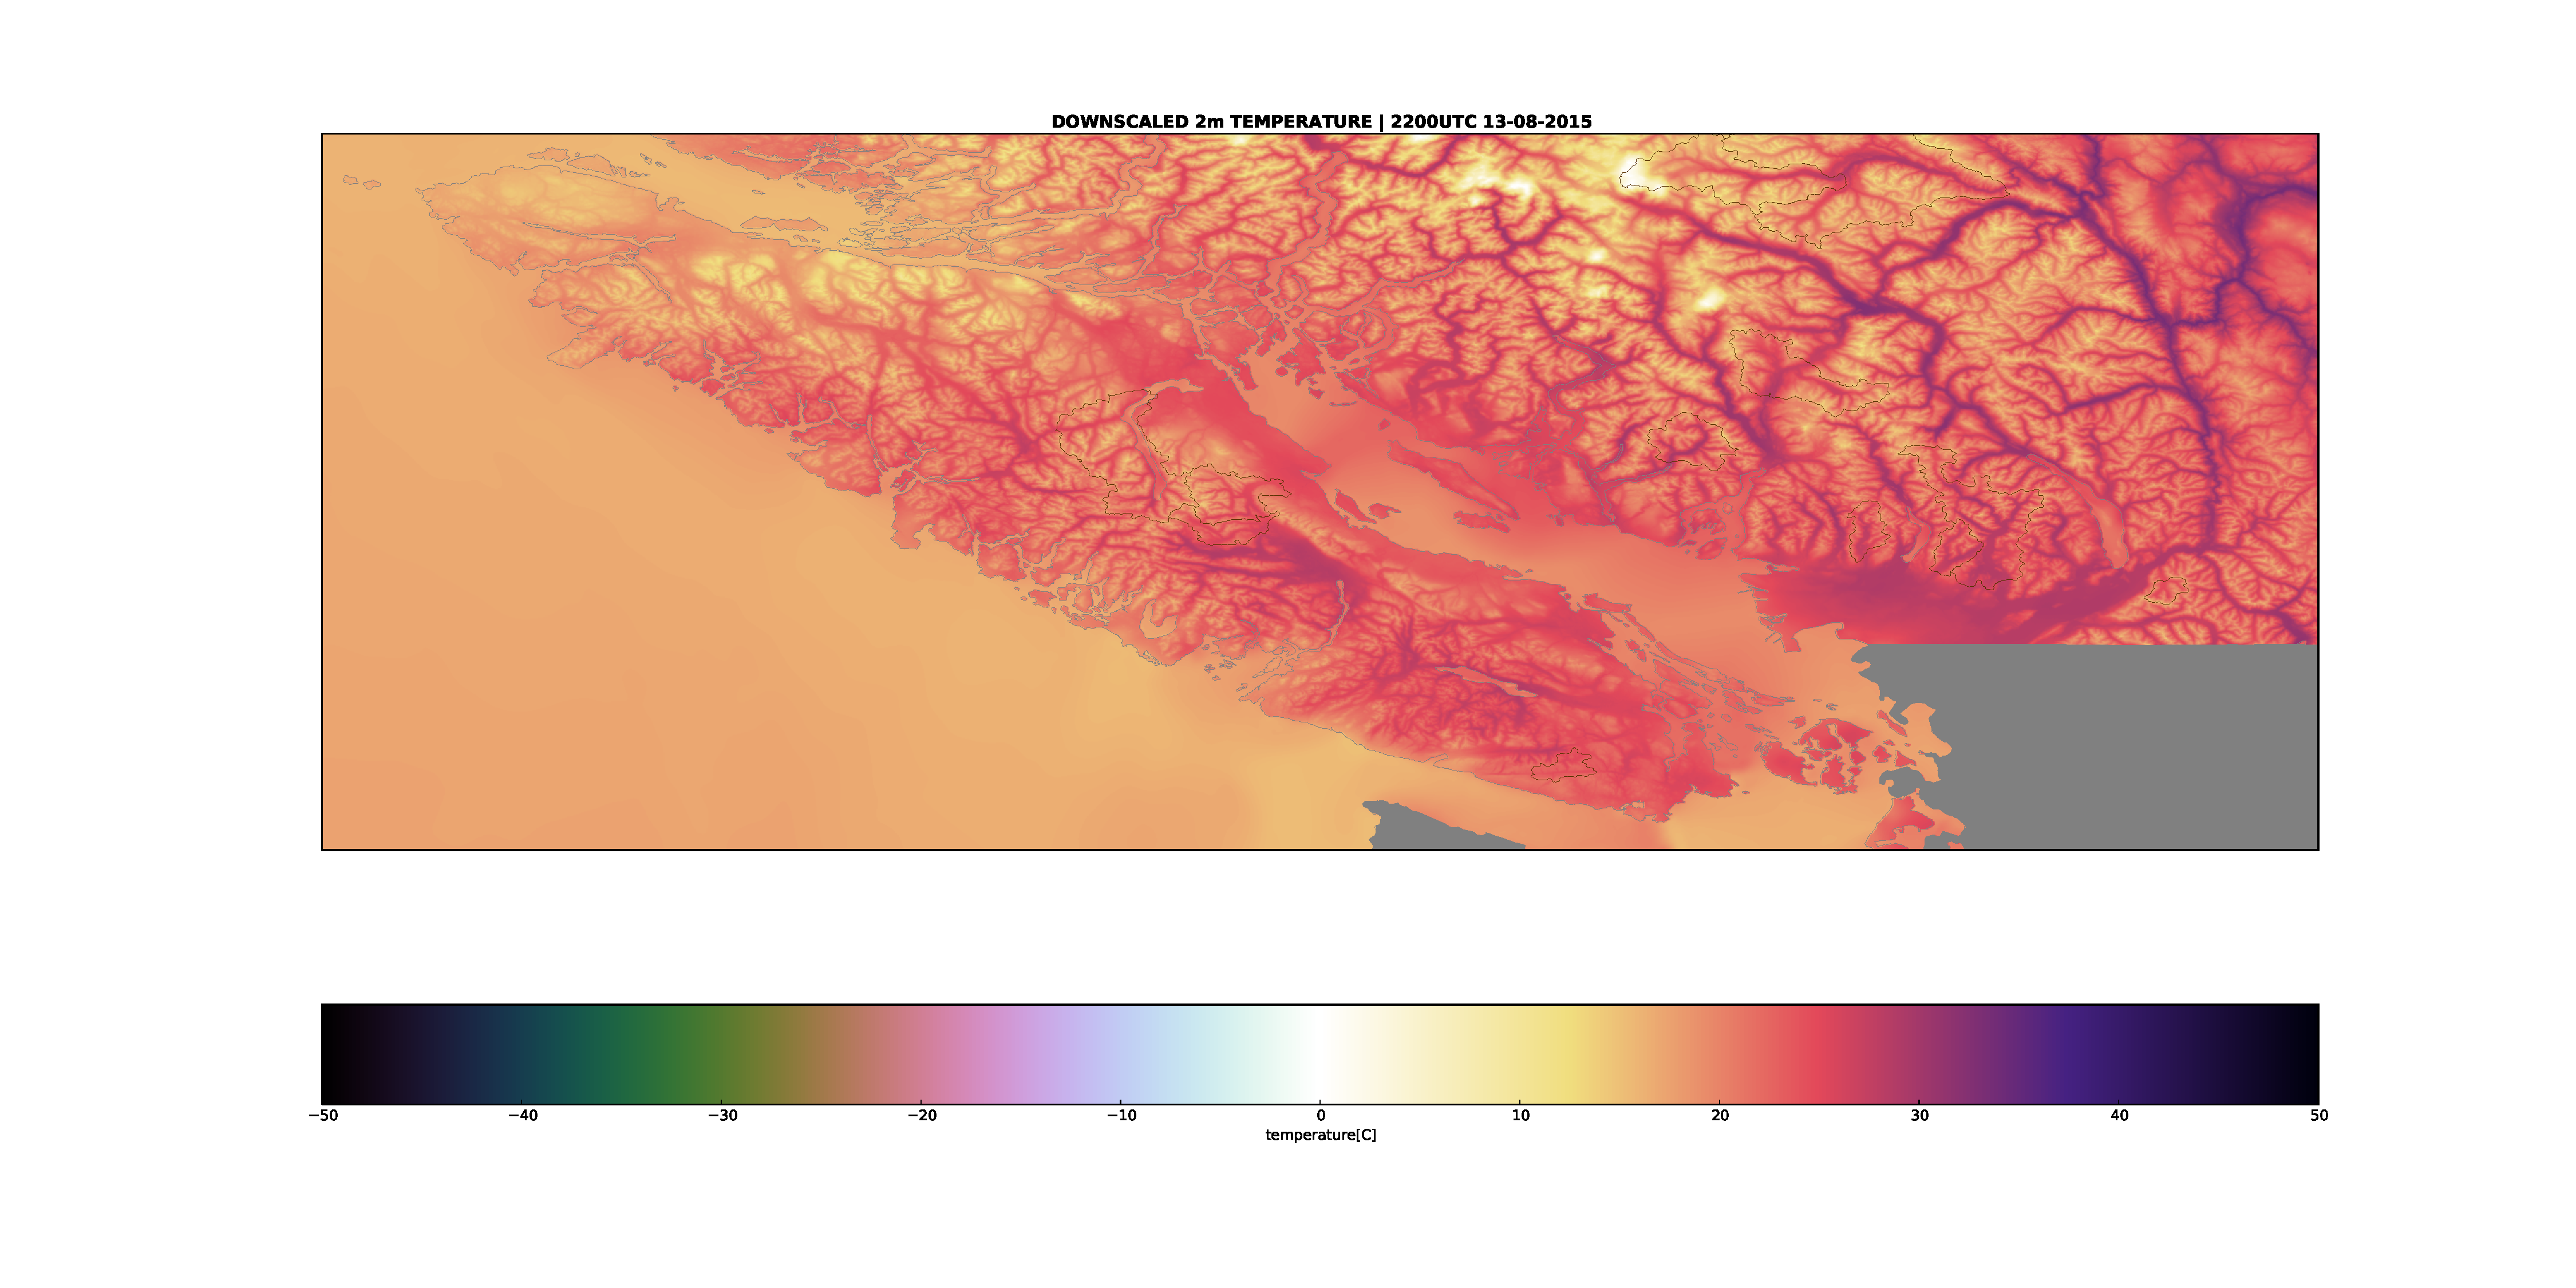
\includegraphics[width=12in]{./graphics/Downscaled_T2_2015-08-13_22.pdf} }
\caption{Downscaled 2m temperature. Gray region masks US territory (no available DEM data). Fine black contours mark BC Hydro watersheds, as designated by Major Hydro Watersheds Project.}\label{fig:downscaledT}
\end{figure}

\begin{figure}
\makebox[\textwidth][c]{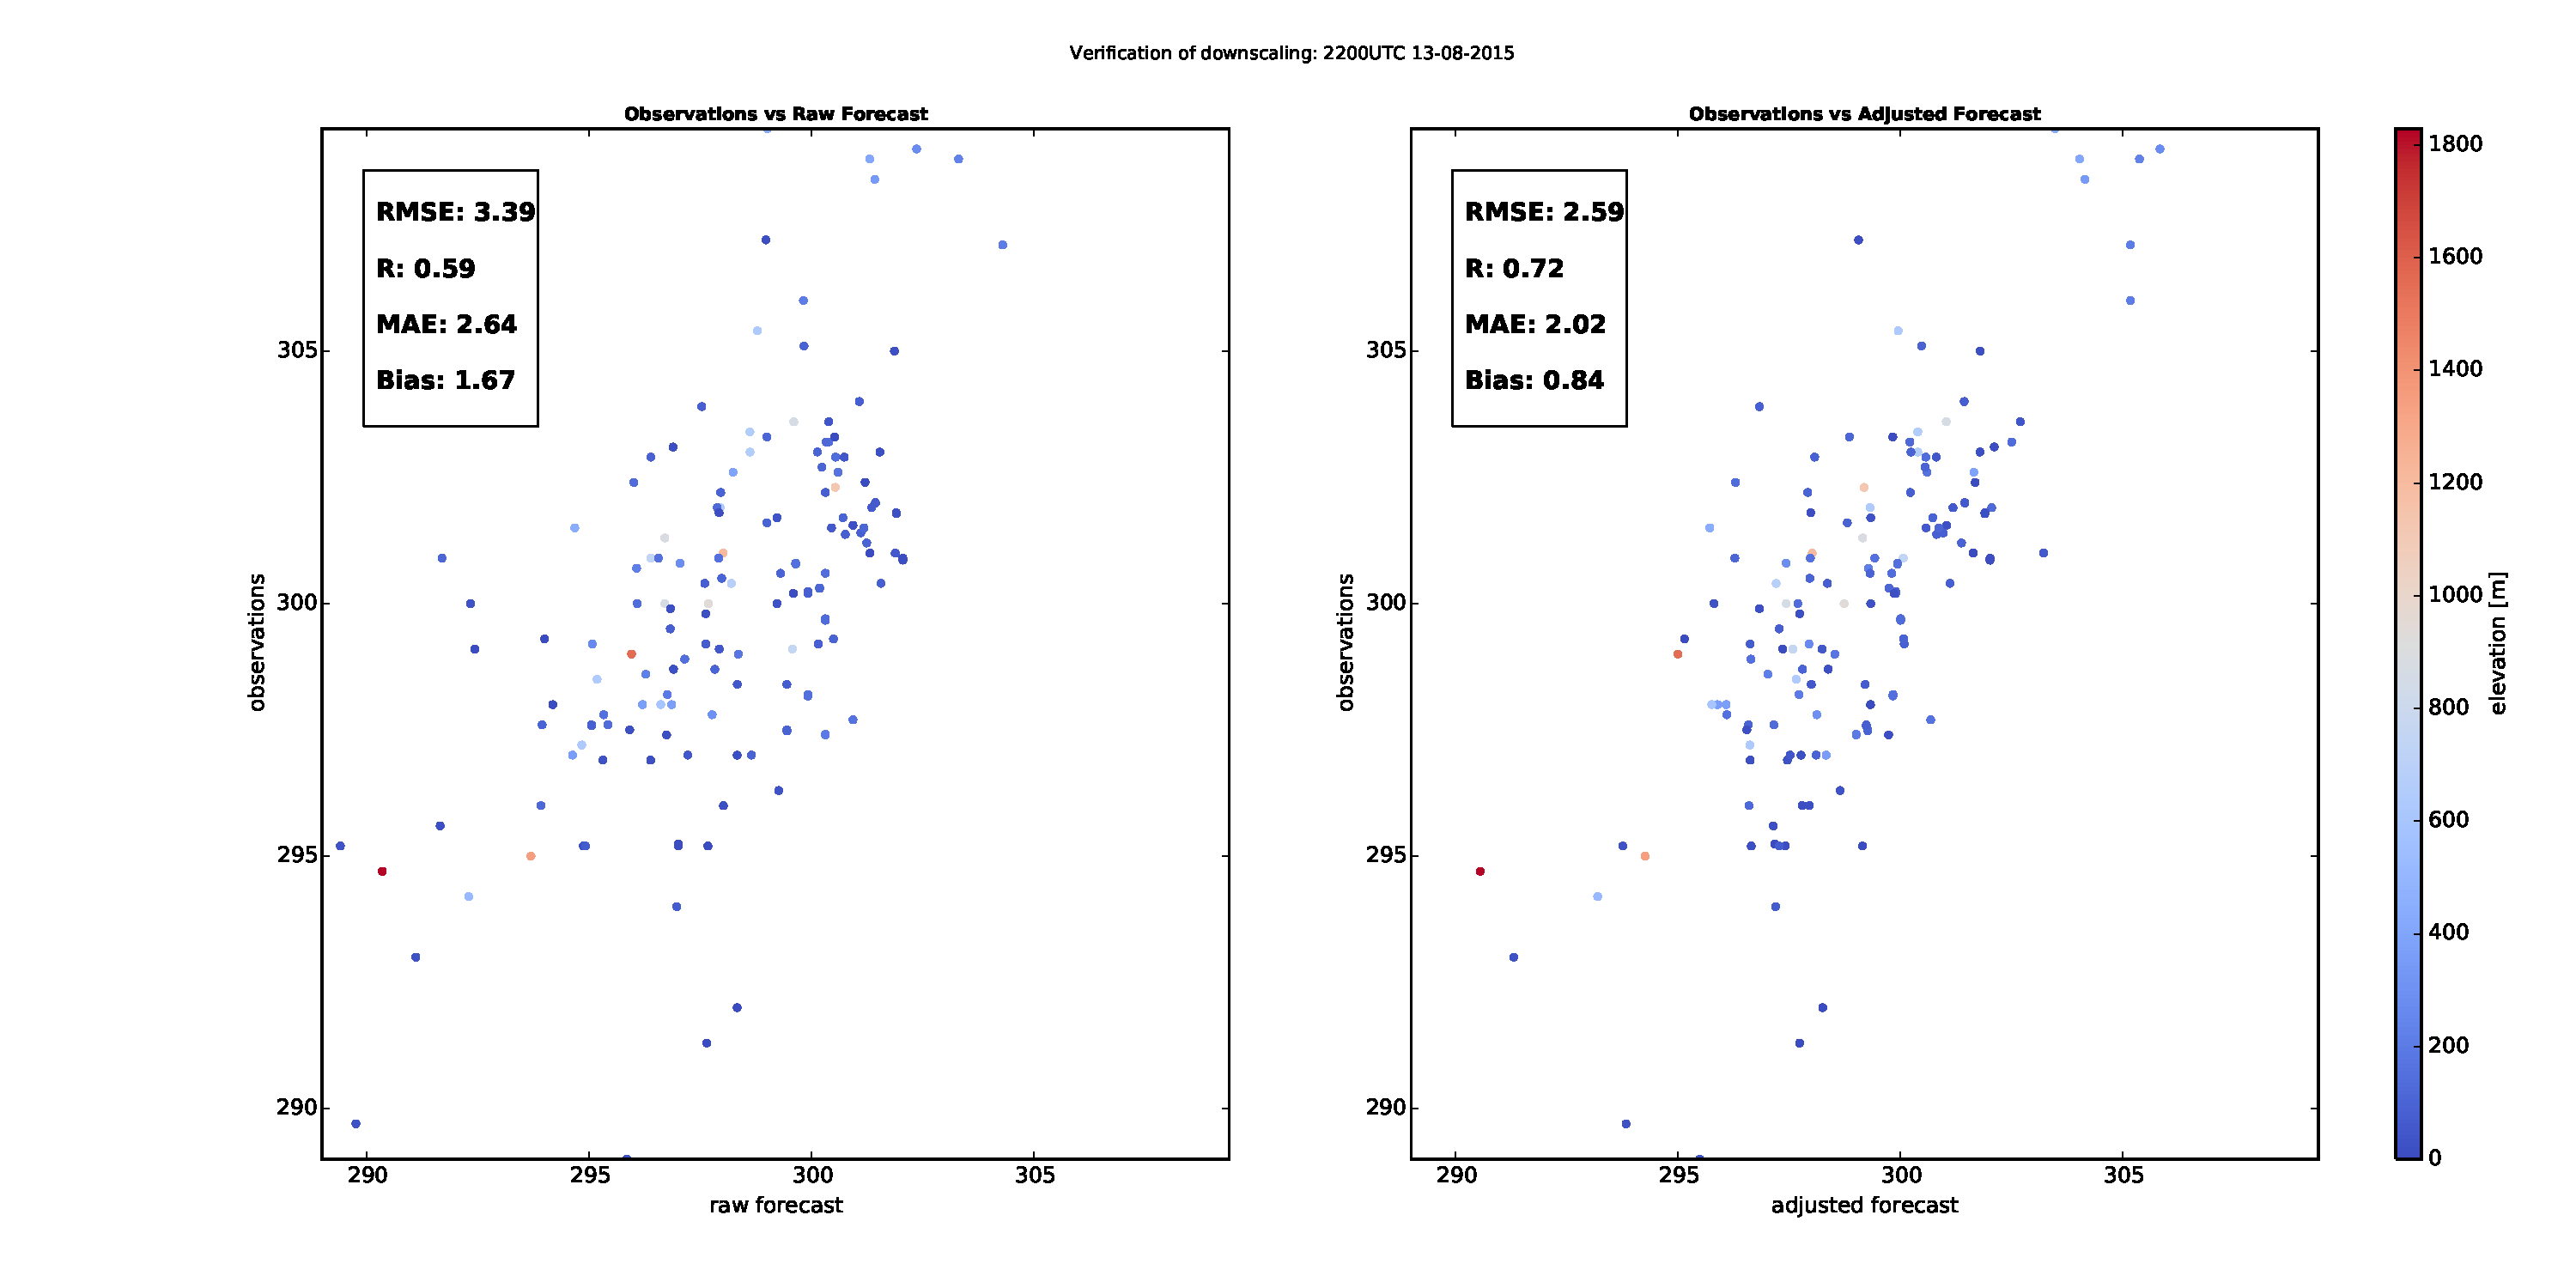
\includegraphics[width=11in]{./graphics/Downscaled_verif_T2_2015-08-13_22.pdf} }
\caption{Downscaling evaluation scatter graphs shown for Raw vs. Observed and Downscaled vs. Observed temperatures. Marker colors correspond to the elevation of observation stations. Also shown: root mean squared error (RMSE), correlation coefficient (R), mean absolute error (MAE) and bias.}\label{fig:verifDS}
\end{figure}

\begin{figure}
\makebox[\textwidth][c]{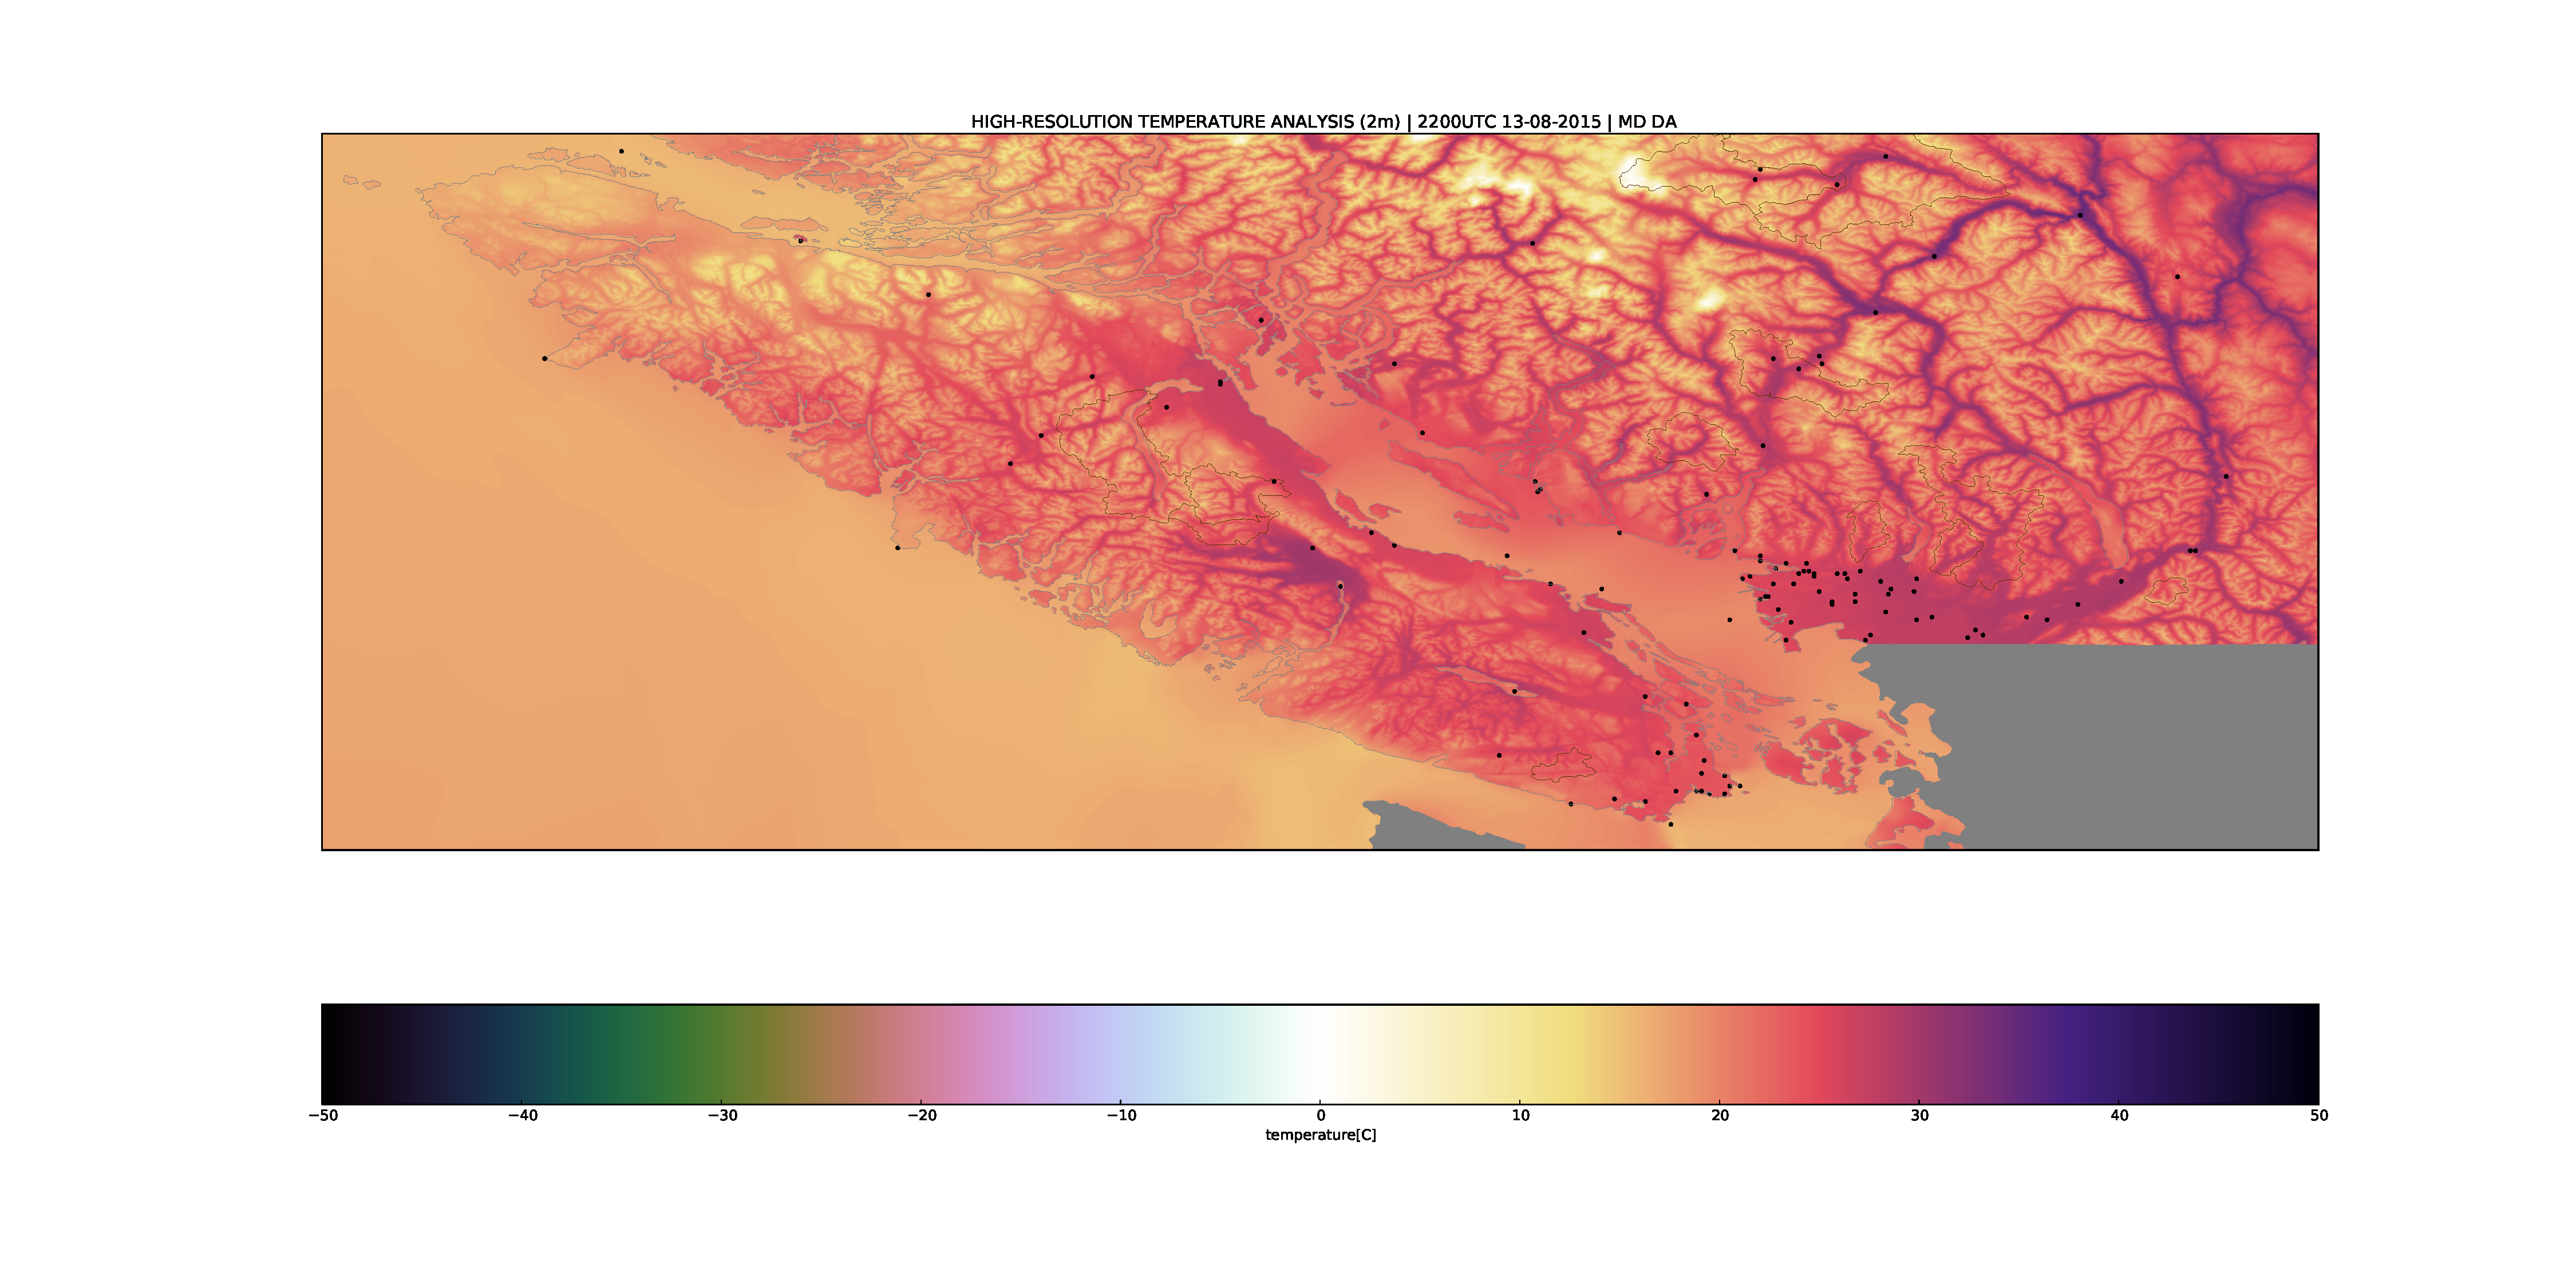
\includegraphics[width=12in]{./graphics/Corrected_T2_2015-08-13_22.pdf} }
\caption{Corrected 2m temperature, based on MD data assimilation approach. Gray region masks US territory (no available DEM data). Fine black contours mark BC Hydro watersheds, as designated by Major Hydro Watersheds Project.}\label{fig:correctedT}
\end{figure}

\begin{figure}
\makebox[\textwidth][c]{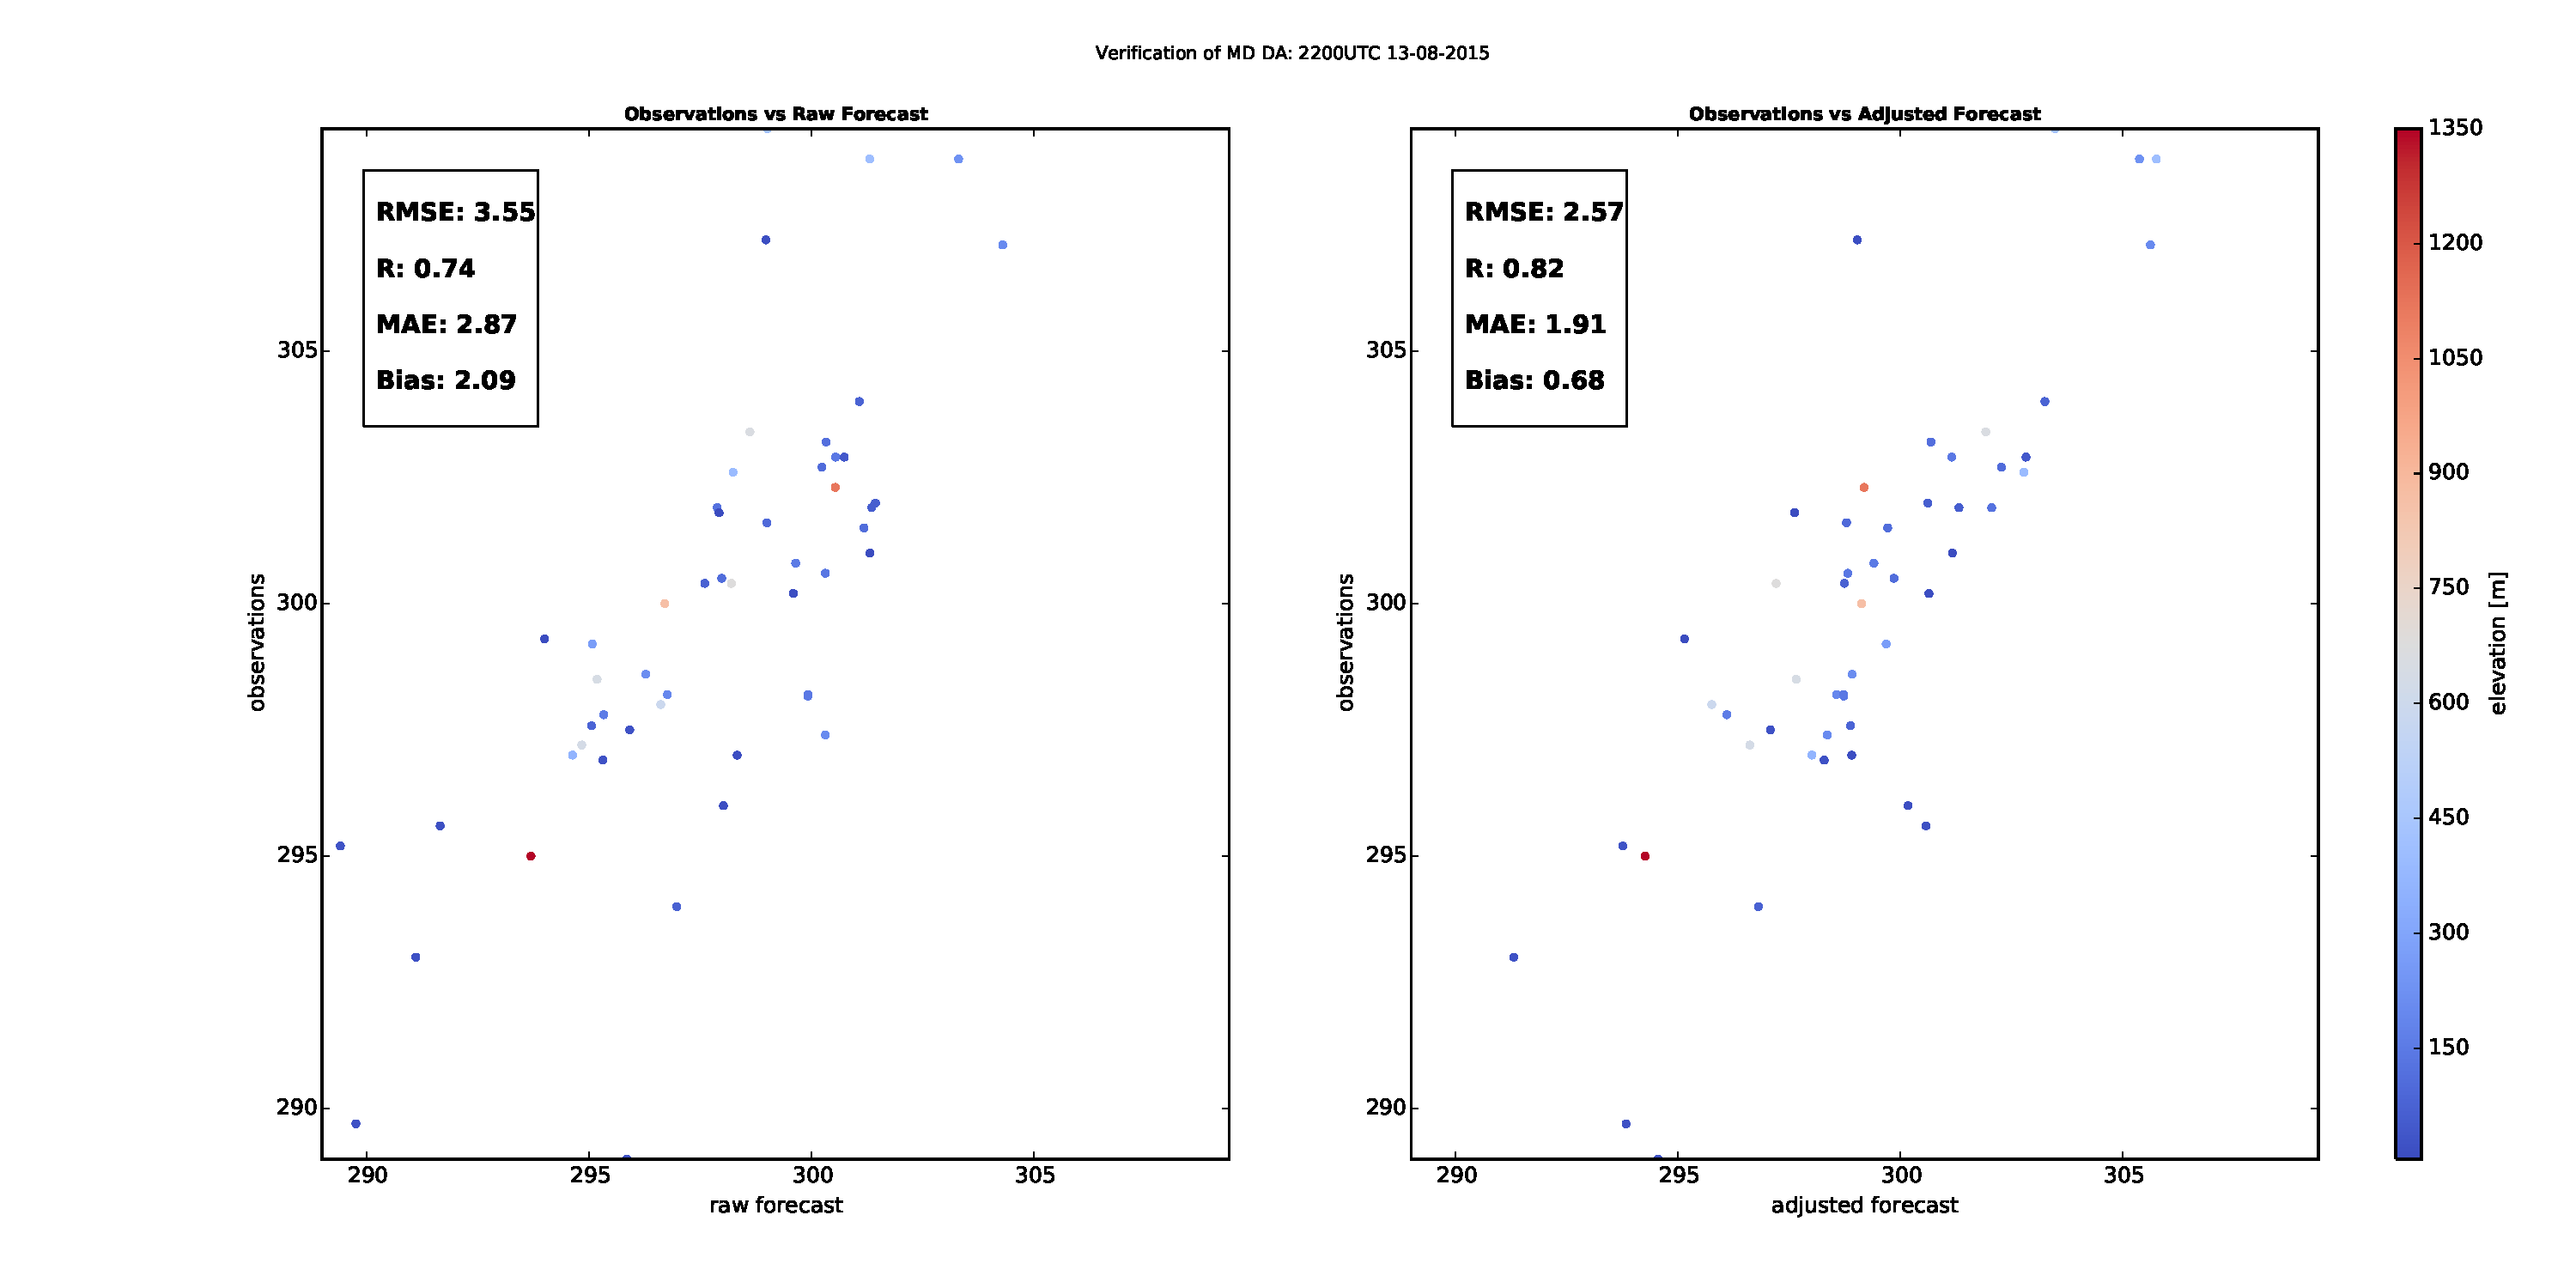
\includegraphics[width=11in]{./graphics/Corrected_verif_T2_2015-08-13_22.pdf} }
\caption{Cross-evaluation of high-resolution analysis (downscaling + data assimilation) using an independent test dataset. Raw vs. Observed and Corrected vs. Observed temperatures. Marker colors correspond to the elevation of observation stations. Also shown: root mean squared error (RMSE), correlation coefficient (R), mean absolute error (MAE) and bias. }\label{fig:verifDA}
\end{figure}

\end{landscape}
\restoregeometry
\pagestyle{plain}
\FloatBarrier

\newpage
\bibliographystyle{elsarticle-harv}
\bibliography{UserManual}




\end{document}

